% \iffalse meta-comment
%
% File: duckuments.dtx Copyright (C) 2018 Jonathan P. Spratte
%
% It may be distributed and/or modified under the conditions of the LaTeX
% Project Public License (LPPL), either version 1.3c of this license or (at your
% option) any later version.  The latest version of this license is in the file
%
%   https://www.latex-project.org/lppl.txt
%
% ------------------------------------------------------------------------------
%
%<*driver>
\def\nameofplainTeX{plain}
\ifx\fmtname\nameofplainTeX\else
  \expandafter\begingroup
\fi
\input l3docstrip.tex
\askforoverwritefalse
\preamble

--------------------------------------------------------------
duckuments -- minimal working duckuments
E-mail: jspratte@yahoo.de
Released under the LaTeX Project Public License v1.3c or later
See http://www.latex-project.org/lppl.txt
--------------------------------------------------------------

Copyright (C) 2018 Jonathan P. Spratte

This  work may be  distributed and/or  modified under  the conditions  of the
LaTeX Project Public License (LPPL),  either version 1.3c  of this license or
(at your option) any later version.  The latest version of this license is in
the file:

  http://www.latex-project.org/lppl.txt

This work is "maintained" (as per LPPL maintenance status) by
  Jonathan P. Spratte.

This work consists of the file  duckuments.dtx
and the derived files           duckuments.pdf,
                                duckuments.sty and
                                example-image-duck.tex

\endpreamble
% stop docstrip adding \endinput
\postamble
\endpostamble
\generate{\file{duckuments.sty}{\from{duckuments.dtx}{pkg}}}
\generate{\file{example-image-duck.tex}{\from{duckuments.dtx}{eid}}}
\ifx\fmtname\nameofplainTeX
  \expandafter\endbatchfile
\else
  \expandafter\endgroup
\fi
%</driver>
%
%<*driver|pkg>
\RequirePackage{xparse,letltxmacro,l3keys2e}
%</driver|pkg>
%
%<*driver>
\ProvidesFile{duckuments.dtx}[2018/03/13 minimal working duckuments]
\documentclass{l3doc}
\usepackage{enumitem}
\newenvironment{options}
  {\begin{description}[style=nextline,font=\normalfont\ttfamily]}
  {\end{description}}
\begin{document}
  \DocInput{duckuments.dtx}
\end{document}
%</driver>
%
%<*eid>
\documentclass[tikz,multi]{standalone}

\usepackage{tikzducks}
\usepackage{duckuments}

\begin{document}
\makeatletter
\foreach\x in {1,2,...,\duckuments@randoms}
  {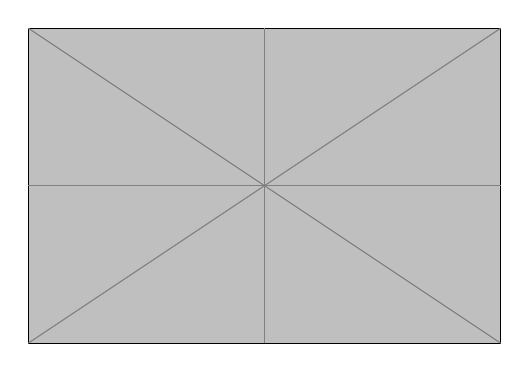
\begin{tikzpicture}
    \draw[black,fill=gray!50] (0,0) rectangle (6,4);
      \draw[gray,thin] (0,0) -- (6,4);
      \draw[gray,thin] (0,4) -- (6,0);
      \draw[gray,thin] (3,0) -- (3,4);
      \draw[gray,thin] (0,2) -- (6,2);
      \node at (3,2) {\tikz\randuck;};
  \end{tikzpicture}}
\makeatother
\end{document}
%</eid>
%
%<*pkg>
\def\duckuments@version{v0.1}
\def\duckuments@date{2018/03/13}
\ProvidesExplPackage
  {duckuments}          {\duckuments@date}
  {\duckuments@version} {minimal working duckuments}
%</pkg>
% \fi
%
% \title{The \pkg{duckuments} package}
% \author{Jonathan P. Spratte\thanks{E-mail: jspratte@yahoo.de}}
% \date{Released 2018/03/13}
% \maketitle
% \tableofcontents
%
% \begin{documentation}
%
% \section{Introduction}
%
% This package was inspired by the question
% \href{https://tex.stackexchange.com/questions/419751}
% {getting ducks in example images}.
% It began on the idea to patch \cs{includegraphics} to automatically change its
% behaviour if |example-image-duck| is used, but then it turned out to be a
% simple alternative to the \pkg{blindtext} package.
%
% It is written as a docstrip file: executing |latex duckuments.dtx| generates
% the \file{duckuments.sty} and \file{example-image-duck.tex} file and typesets
% this duckumentation; execute |tex duckuments.dtx| to only generate the files
% \file{duckuments.sty} and \file{example-image-duck.tex}.
%
% For its functionality \file{example-image-duck.tex} must be compiled at least
% once. The package does currently only work on \pdfTeX\ and \LuaTeX.
%
% The sources are hosted on
% \href{https://github.com/Skillmon/ltx_duckuments}{github}.
%
% \section{Duckumentation}
%
% \subsection{Dummy content}
%
% \begin{function}{\duckument}
%   \begin{syntax}
%     \cs{duckument}\oarg{key=value}
%   \end{syntax}
%   Produces a duckument with one sectioning entry of each level starting at
%   \cs{chapter} (if available) and two variants of the list environment
%   \env{itemize}, \env{enumerate}, and \env{description}, one only at top
%   level and one with 4~environments nested. The \meta{key=value}s accept every
%   key as explained in \autoref{sec:keys}, but not every key has an effect.
% \end{function}
%
% \begin{function}{\blindduck}
%   \begin{syntax}
%     \cs{blindduck}\oarg{key=value}
%   \end{syntax}
%   Produces one paragraph of dummy content. The \meta{key=value}s accept every
%   key as explained in \autoref{sec:keys}, but not every key has an effect.
% \end{function}
%
% \begin{function}{\blindlist}
%   \begin{syntax}
%     \cs{blindlist}\meta{*}\marg{environment}
%   \end{syntax}
%   Sets a list of the specified \meta{environment}, if \meta{*} is given
%   \cs{item}\oarg{dummy} is used instead of only \cs{item}. For |description|
%   the starred version is used automatically.
% \end{function}
%
% \begin{function}{\blindlistlist}
%   \begin{syntax}
%     \cs{blindlistlist}\meta{*}\marg{list}
%   \end{syntax}
%   Sets 4~levels of a nested list of the specified \meta{environment}, if
%   \meta{*} is given \cs{item}\oarg{dummy} is used instead of only \cs{item}.
%   For |description| the starred version is used automatically.
% \end{function}
%
% \begin{function}{\duckitemize}
%   Abbreviation for \cs{ducklist}|{itemize}|.
% \end{function}
%
% \begin{function}{\duckenumerate}
%   Abbreviation for \cs{ducklist}|{enumerate}|.
% \end{function}
%
% \begin{function}{\duckdescription}
%   Abbreviation for \cs{ducklist}|{description}|.
% \end{function}
%
% \subsection{Patches}
%
% The package patches \cs{includegraphics} if it is defined at the time the
% patch is applied (see \autoref{sec:keys}, |immediate|). The patch changes the
% behaviour if |example-image-duck| is used. If that is the case, a random page
% of that document is used. There shouldn't be any change in behaviour if other
% files are used.
%
% The patch is done so that one can use \pkg{tikzducks} ducks without the need
% of loading \pkg{tikz} in a minimal working duckument as example images.
%
% \subsection{Options}\label{sec:keys}
%
% The package and commands which take a \oarg{key=value} accept the following
% options. Some of which only make sense as package options. The
% \textbf{\texttt{bold}} printed value is the one used if you don't specify a
% value.
% \begin{options}
%   \item[toc=\textbf{true}$\vert$false]
%     If |true| the \cs{duckument} contains a ToC.
%   \item[maths=\textbf{both}$\vert$inline$\vert$display$\vert$none]
%     If |both| the \cs{blindduck} (which is also used by \cs{duckument})
%     contains both inline and displayed math. With |inline| and |display| the
%     respective maths is activated. |none| disables both.
%   \item[immediate=\textbf{true}$\vert$false]
%     If |true| \cs{includegraphics} is patched during package load time, else
%     the patching is done \cs{AtBeginDocument}.
% \end{options}
%
% \end{documentation}
%
% \begin{implementation}
%
% \section{Implementation}
%
%    \begin{macrocode}
%<*pkg>
%    \end{macrocode}
% 
%    \begin{macrocode}
%<@@=duckuments>
%    \end{macrocode}
%
% \subsection{Check for possible problems}
%
% Check which engine is used.
%    \begin{macrocode}
\bool_if:nF { \sys_if_engine_luatex_p: || \sys_if_engine_pdftex_p: }
  { %>>>
    \msg_new:nnnn { duckuments } { incompatible } 
      {
        The~duckuments~package~is~currently~only~compatible~with~pdfTeX~and~
        LuaTeX!
      }
      {
        Sorry~for~that.
      }
    \msg_error:nn { duckuments } { incompatible }
    \endinput
  }%<<<
%    \end{macrocode}
%
% Check whether \file{example-image-duck.pdf} exists.
%    \begin{macrocode}
\file_if_exist:nF { example-image-duck.pdf }
  {%>>>
%    \end{macrocode}
% If the current \cs{jobname} doesn't match \file{example-image-duck} throw a
% warning.
%    \begin{macrocode}
    \str_if_eq:VnF \c_sys_jobname_str { example-image-duck }
      {
        \msg_new:nnnn { duckuments } { missing-file }
        {
          The~file~`#1`~can't~be~found.~Make~sure~to~create~it
          \tl_if_empty:nF{#2}{~#2}.
        }
        { Sorry~for~the~inconvenience. }
        \msg_warning:nnnn { duckuments } { missing-file }
          { example-image-duck.pdf }
          { by~compiling~example-image-duck.tex~at~least~once }
      }
  }%<<<
%    \end{macrocode}
%
% \subsection{Variables}
%
% \begin{variable}{\duckuments@randoms}
%   Stores the number of random ducks in \file{example-image-duck.pdf}.
%    \begin{macrocode}
\newcommand*\duckuments@randoms{100}
%    \end{macrocode}
% \end{variable}
%
%
% \begin{variable}{\l_duckuments_immediate_bool}
%   Stores whether the patch is to be done during package load time.
%    \begin{macrocode}
\bool_new:N \l_duckuments_immediate_bool
%    \end{macrocode}
% \end{variable}
%
% \begin{variable}{\l_duckuments_toc_bool}
%   Stores whether to display a ToC in \cs{duckument}.
%    \begin{macrocode}
\bool_new:N \l_duckuments_toc_bool
%    \end{macrocode}
% \end{variable}
%
% \begin{variable}{\l_duckuments_math_inline_bool}
%   Stores whether to display inline math in \cs{blindduck}.
%    \begin{macrocode}
\bool_new:N \l_duckuments_math_inline_bool
%    \end{macrocode}
% \end{variable}
%
% \begin{variable}{\l_duckuments_math_display_bool}
%   Stores whether to display displayed math in \cs{blindduck}.
%    \begin{macrocode}
\bool_new:N \l_duckuments_math_display_bool
%    \end{macrocode}
% \end{variable}
%
% \subsection{Constants}
%
% \begin{variable}{\c_duckuments_regex}
%   Regex against which the patch of \cs{includegraphics} is testing.
%    \begin{macrocode}
\regex_const:Nn \c_duckuments_regex
  { example-image-duck|example-image-duck.pdf }
%    \end{macrocode}
% \end{variable}
%
% \subsection{Options and Configurations}
%    \begin{macrocode}
\keys_define:nn { duckuments }
  {%>>>
    ,toc   .bool_set:N = \l_duckuments_toc_bool
    ,toc   .default:n = true
    ,maths .choice:
    ,maths / both    .code:n =
      {
        \bool_set_true:N \l_duckuments_math_inline_bool
        \bool_set_true:N \l_duckuments_math_display_bool
      }
    ,maths / none    .code:n =
      {
        \bool_set_false:N \l_duckuments_math_inline_bool
        \bool_set_false:N \l_duckuments_math_display_bool
      }
    ,maths / inline  .code:n = \bool_set_true:N \l_duckuments_math_inline_bool
    ,maths / display .code:n = \bool_set_true:N \l_duckuments_math_display_bool
    ,maths .default:n = both
    ,immediate .bool_set:N = \l_duckuments_immediate_bool
    ,immediate .default:n = true
  }%<<<
\ProcessKeysOptions { duckuments }
\bool_if:NTF \l_duckuments_immediate_bool
  { \AtEndOfPackage { \duckuments_patch_includegraphics: } }
  { \AtBeginDocument { \duckuments_patch_includegraphics: } }
%    \end{macrocode}
%
% \subsection{Functions}
%
% \subsubsection{Duckument Level}
%
% \begin{macro}{\duckument}
%    \begin{macrocode}
\NewDocumentCommand \duckument { O{} }
  {%>>>
    \group_begin:
    \keys_set:nn { duckuments } { #1 }
    \bool_if:NT \l_duckuments_toc_bool { \tableofcontents }
    \cs_if_exist_use:NT \chapter
      { {\duckuments@headings@text{0}} \blindduck }
    \duckuments@headings{1} \blindduck
    \duckuments@headings{2} \blindduck
    \duckuments@headings{3} \blindduck
    \duckuments@headings{4} \blindduck
    \section {Lists}
    \duckuments_list_example:n { itemize }
    \duckuments_list_example:n { enumerate }
    \duckuments_list_example:n { description }
    \group_end:
  }%<<<
%    \end{macrocode}
% \end{macro}
%
% \begin{macro}{\blindduck}
%    \begin{macrocode}
\NewDocumentCommand \blindduck { O{} }
  {%>>>
    \group_begin:
    \keys_set:nn { duckuments } { #1 }
    \duckuments@blindduck@text
    \group_end:
  }%<<<
%    \end{macrocode}
% \end{macro}
%
% \begin{macro}{\blindlist}
%    \begin{macrocode}
\NewDocumentCommand \ducklist {s m}
  {%>>>
    \begin{#2}
      \IfBooleanTF { #1 }
        {\ducklists@content@starred}
        {
          \str_if_eq:nnTF { #2 } { description }
            \ducklists@content@starred
            \ducklists@content
        }
    \end{#2}
  }%<<<
%    \end{macrocode}
% \end{macro}
%
% \begin{macro}{\blindlistlist}
%    \begin{macrocode}
\NewDocumentCommand \ducklistlist { s m }
  {%>>>
    \IfBooleanTF { #1 }
      { \duckuments@listlist@starred { #2 } }
      {
        \str_if_eq:nnTF { #2 } { description }
          { \duckuments@listlist@starred { description } }
          { \duckuments@listlist{#2} }
      }
  }%<<<
%    \end{macrocode}
% \end{macro}
%
%
% \begin{macro}{\duckenumerate}
%    \begin{macrocode}
\newcommand*\duckenumerate{\ducklist{enumerate}}
%    \end{macrocode}
% \end{macro}
% \begin{macro}{\duckitemize}
%    \begin{macrocode}
\newcommand*\duckitemize{\ducklist{itemize}}
%    \end{macrocode}
% \end{macro}
% \begin{macro}{\duckdescription}
%    \begin{macrocode}
\newcommand*\duckdescription{\ducklist{description}}
%    \end{macrocode}
% \end{macro}
%
% \subsubsection{Intern}
%
% \begin{macro}{\duckuments@headings}
%    \begin{macrocode}
\newcommand*\duckuments@headings[1]
  {%>>>
    \ifcase#1\relax
      \expandafter\chapter
    \or \expandafter\section
    \or \expandafter\subsection
    \or \expandafter\subsubsection
    \or \expandafter\paragraph
    \else \expandafter\@gobble
    \fi
    {\duckuments@headings@text{#1}}
  }%<<<
%    \end{macrocode}
% \end{macro}
%
% \begin{macro}{\duckuments@headings@level}
%    \begin{macrocode}
\newcommand*\duckuments@headings@level[1]
  {%>>>
    (
    \ifcase#1
      chapter
    \or section
    \or subsection
    \or subsubsection
    \or paragraph
    \fi
    )
  }%<<<
%    \end{macrocode}
% \end{macro}
%
% \begin{macro}{\duckuments@ifinline}
%    \begin{macrocode}
\newcommand*\duckuments@ifinline[2][]
  { \bool_if:NTF \l_duckuments_math_inline_bool { #2 } { #1 } }
%    \end{macrocode}
% \end{macro}
%
% \begin{macro}{\duckuments@ifdisplay}
%    \begin{macrocode}
\newcommand*\duckuments@ifdisplay[2][]
  { \bool_if:NTF \l_duckuments_math_display_bool { #2 } { #1 } }
%    \end{macrocode}
% \end{macro}
%
% \begin{macro}{\duckuments_list_example:n}
%    \begin{macrocode}
\cs_new_protected_nopar:Nn \duckuments_list_example:n
  {%>>>
    \subsection{Example\ for\ ducks\ (#1)}
    \ducklist { #1 }
    \subsubsection{Nested\ ducks}
    \ducklistlist { #1 }
  }%<<<
%    \end{macrocode}
% \end{macro}
%
% \begin{macro}{\duckuments@enquote}
%    \begin{macrocode}
\newcommand*\duckuments@enquote [1]
  {%>>>
    \cs_if_exist_use:NTF
      \enquote { #1 }
      {``#1''}
  }%<<<
%    \end{macrocode}
% \end{macro}
%
% \begin{macro}{\duckuments_patch_includegraphics:}
%    \begin{macrocode}
\cs_new_protected_nopar:Nn \duckuments_patch_includegraphics:
  {%>>>
    \cs_if_exist:NT \includegraphics
      {
        \LetLtxMacro\duckuments@includegraphicsBAK\includegraphics
        \RenewDocumentCommand \includegraphics
          { >{\duckuments_starred:n}s O{} m }
          {
            \regex_match:NnTF \c_duckuments_regex { ##3 }
              {
                \duckuments@includegraphicsBAK##1
                  [page=\int_rand:nn{1}{\duckuments@randoms},##2] { ##3 }
              }
              {
                \duckuments@includegraphicsBAK##1[##2]{##3}
              }
          }
      }
  }%<<<
%    \end{macrocode}
% \end{macro}
%
% \begin{macro}{\duckuments_starred:n}
%    \begin{macrocode}
\cs_new_protected:Nn \duckuments_starred:n
  {%>>>
    \IfBooleanTF { #1 }
      { \def\ProcessedArgument{*} }
      { \def\ProcessedArgument{} } 
  }%<<<
%    \end{macrocode}
% \end{macro}
%
%    \begin{macrocode}
\ExplSyntaxOff
%    \end{macrocode}
%
% \begin{macro}{\duckuments@blindduck@text}
%    \begin{macrocode}
\newcommand*\duckuments@blindduck@text
  {%>>>
    There once was a very smart but sadly blind duck. When it was still a small
    duckling it was renowned for its good vision. But sadly as the duck grew
    older it caught a sickness which caused its eyesight to worsen. It became so
    bad, that the duck couldn't read the notes it once took containing much of
    inline math\duckuments@ifinline{ just like its favoured equation: $d = u_c
    \cdot k$}. Only displayed equations remained legible%
    \duckuments@ifdisplay[.]{ so it could still read \begin{equation}d = r a^k
    e\hbox{.}\end{equation}} That annoyed the smart duck, as it wasn't able to
    do its research any longer. It called for its underduckling and said:
    \duckuments@enquote{Go, find me the best eye ducktor there is. He shall
    heal me from my disease!}%
  }%<<<
%    \end{macrocode}
% \end{macro}
%
% \begin{macro}{\duckuments@headings@text}
%    \begin{macrocode}
\newcommand*\duckuments@headings@text[1]
  {A friendly duck at level #1 \duckuments@headings@level{#1}}
%    \end{macrocode}
% \end{macro}
%
% \begin{macro}{\ducklists@content}
%    \begin{macrocode}
\newcommand*\ducklists@content
  {%>>>
    \item First swims father drake
    \item Then floats mother duck
    \item After her paddles baby duckling
    \item And over there bathes uncle canard
  }%<<<
%    \end{macrocode}
% \end{macro}
%
% \begin{macro}{\ducklists@content@starred}
%    \begin{macrocode}
\newcommand*\ducklists@content@starred
  {%>>>
    \item[drake] is the swimming father
    \item[duck] is the floating mother
    \item[duckling] is the paddling baby
    \item[canard] is the bathing uncle
  }%<<<
%    \end{macrocode}
% \end{macro}
%
% \begin{macro}{\duckuments@listlist}
%    \begin{macrocode}
\newcommand*\duckuments@listlist[1]
  {%>>>
    \begin{#1}
      \item swimming father drake
        \begin{#1}
          \item swimming father drake
            \begin{#1}
              \item swimming father drake
                \begin{#1}
                  \item swimming father drake
                  \item floating mother duck
                \end{#1}
              \item floating mother duck
            \end{#1}
          \item floating mother duck
        \end{#1}
      \item floating mother duck
    \end{#1}%
  }%<<<
%    \end{macrocode}
% \end{macro}
%
% \begin{macro}{\duckuments@listlist@starred}
%    \begin{macrocode}
\newcommand*\duckuments@listlist@starred[1]
  {%>>>
    \begin{#1}
      \item[drake] is the swimming father
        \begin{#1}
          \item[drake] is the swimming father
            \begin{#1}
              \item[drake] is the swimming father
                \begin{#1}
                  \item[drake] is the swimming father
                  \item[duck] is the floating mother
                \end{#1}
              \item[duck] is the floating mother
            \end{#1}
          \item[duck] is the floating mother
        \end{#1}
      \item[duck] is the floating mother
    \end{#1}%
  }%<<<
%    \end{macrocode}
% \end{macro}
%
%    \begin{macrocode}
\endinput
%    \end{macrocode}
%
% \end{implementation}
%
%    \begin{macrocode}
%</pkg>
%    \end{macrocode}
%
%^^A vim: fdm=marker foldmarker=>>>,<<<
